\documentclass[]{report}
\usepackage{lmodern}
\usepackage{amssymb,amsmath}
\usepackage{ifxetex,ifluatex}
\usepackage{fixltx2e} % provides \textsubscript
\ifnum 0\ifxetex 1\fi\ifluatex 1\fi=0 % if pdftex
  \usepackage[T1]{fontenc}
  \usepackage[utf8]{inputenc}
\else % if luatex or xelatex
  \ifxetex
    \usepackage{mathspec}
  \else
    \usepackage{fontspec}
  \fi
  \defaultfontfeatures{Ligatures=TeX,Scale=MatchLowercase}
\fi
% use upquote if available, for straight quotes in verbatim environments
\IfFileExists{upquote.sty}{\usepackage{upquote}}{}
% use microtype if available
\IfFileExists{microtype.sty}{%
\usepackage{microtype}
\UseMicrotypeSet[protrusion]{basicmath} % disable protrusion for tt fonts
}{}
\usepackage{hyperref}
\hypersetup{unicode=true,
            pdftitle={PROJECT 2: PREDICTING PH},
            pdfauthor={Juliann McEachern},
            pdfborder={0 0 0},
            breaklinks=true}
\urlstyle{same}  % don't use monospace font for urls
\usepackage{color}
\usepackage{fancyvrb}
\newcommand{\VerbBar}{|}
\newcommand{\VERB}{\Verb[commandchars=\\\{\}]}
\DefineVerbatimEnvironment{Highlighting}{Verbatim}{commandchars=\\\{\}}
% Add ',fontsize=\small' for more characters per line
\usepackage{framed}
\definecolor{shadecolor}{RGB}{248,248,248}
\newenvironment{Shaded}{\begin{snugshade}}{\end{snugshade}}
\newcommand{\AlertTok}[1]{\textcolor[rgb]{0.94,0.16,0.16}{#1}}
\newcommand{\AnnotationTok}[1]{\textcolor[rgb]{0.56,0.35,0.01}{\textbf{\textit{#1}}}}
\newcommand{\AttributeTok}[1]{\textcolor[rgb]{0.77,0.63,0.00}{#1}}
\newcommand{\BaseNTok}[1]{\textcolor[rgb]{0.00,0.00,0.81}{#1}}
\newcommand{\BuiltInTok}[1]{#1}
\newcommand{\CharTok}[1]{\textcolor[rgb]{0.31,0.60,0.02}{#1}}
\newcommand{\CommentTok}[1]{\textcolor[rgb]{0.56,0.35,0.01}{\textit{#1}}}
\newcommand{\CommentVarTok}[1]{\textcolor[rgb]{0.56,0.35,0.01}{\textbf{\textit{#1}}}}
\newcommand{\ConstantTok}[1]{\textcolor[rgb]{0.00,0.00,0.00}{#1}}
\newcommand{\ControlFlowTok}[1]{\textcolor[rgb]{0.13,0.29,0.53}{\textbf{#1}}}
\newcommand{\DataTypeTok}[1]{\textcolor[rgb]{0.13,0.29,0.53}{#1}}
\newcommand{\DecValTok}[1]{\textcolor[rgb]{0.00,0.00,0.81}{#1}}
\newcommand{\DocumentationTok}[1]{\textcolor[rgb]{0.56,0.35,0.01}{\textbf{\textit{#1}}}}
\newcommand{\ErrorTok}[1]{\textcolor[rgb]{0.64,0.00,0.00}{\textbf{#1}}}
\newcommand{\ExtensionTok}[1]{#1}
\newcommand{\FloatTok}[1]{\textcolor[rgb]{0.00,0.00,0.81}{#1}}
\newcommand{\FunctionTok}[1]{\textcolor[rgb]{0.00,0.00,0.00}{#1}}
\newcommand{\ImportTok}[1]{#1}
\newcommand{\InformationTok}[1]{\textcolor[rgb]{0.56,0.35,0.01}{\textbf{\textit{#1}}}}
\newcommand{\KeywordTok}[1]{\textcolor[rgb]{0.13,0.29,0.53}{\textbf{#1}}}
\newcommand{\NormalTok}[1]{#1}
\newcommand{\OperatorTok}[1]{\textcolor[rgb]{0.81,0.36,0.00}{\textbf{#1}}}
\newcommand{\OtherTok}[1]{\textcolor[rgb]{0.56,0.35,0.01}{#1}}
\newcommand{\PreprocessorTok}[1]{\textcolor[rgb]{0.56,0.35,0.01}{\textit{#1}}}
\newcommand{\RegionMarkerTok}[1]{#1}
\newcommand{\SpecialCharTok}[1]{\textcolor[rgb]{0.00,0.00,0.00}{#1}}
\newcommand{\SpecialStringTok}[1]{\textcolor[rgb]{0.31,0.60,0.02}{#1}}
\newcommand{\StringTok}[1]{\textcolor[rgb]{0.31,0.60,0.02}{#1}}
\newcommand{\VariableTok}[1]{\textcolor[rgb]{0.00,0.00,0.00}{#1}}
\newcommand{\VerbatimStringTok}[1]{\textcolor[rgb]{0.31,0.60,0.02}{#1}}
\newcommand{\WarningTok}[1]{\textcolor[rgb]{0.56,0.35,0.01}{\textbf{\textit{#1}}}}
\usepackage{graphicx,grffile}
\makeatletter
\def\maxwidth{\ifdim\Gin@nat@width>\linewidth\linewidth\else\Gin@nat@width\fi}
\def\maxheight{\ifdim\Gin@nat@height>\textheight\textheight\else\Gin@nat@height\fi}
\makeatother
% Scale images if necessary, so that they will not overflow the page
% margins by default, and it is still possible to overwrite the defaults
% using explicit options in \includegraphics[width, height, ...]{}
\setkeys{Gin}{width=\maxwidth,height=\maxheight,keepaspectratio}
\IfFileExists{parskip.sty}{%
\usepackage{parskip}
}{% else
\setlength{\parindent}{0pt}
\setlength{\parskip}{6pt plus 2pt minus 1pt}
}
\setlength{\emergencystretch}{3em}  % prevent overfull lines
\providecommand{\tightlist}{%
  \setlength{\itemsep}{0pt}\setlength{\parskip}{0pt}}
\setcounter{secnumdepth}{0}

%%% Use protect on footnotes to avoid problems with footnotes in titles
\let\rmarkdownfootnote\footnote%
\def\footnote{\protect\rmarkdownfootnote}

%%% Change title format to be more compact
\usepackage{titling}

% Create subtitle command for use in maketitle
\providecommand{\subtitle}[1]{
  \posttitle{
    \begin{center}\large#1\end{center}
    }
}

\setlength{\droptitle}{-2em}

  \title{PROJECT 2: PREDICTING PH}
    \pretitle{\vspace{\droptitle}\centering\huge}
  \posttitle{\par}
    \author{Juliann McEachern}
    \preauthor{\centering\large\emph}
  \postauthor{\par}
      \predate{\centering\large\emph}
  \postdate{\par}
    \date{10 December 2019}

% set plain style for page numbers
\usepackage[margin=1in]{geometry}
\usepackage{fancyhdr}
\pagestyle{fancy}
\fancyhead[LE,RO]{\textbf{Group 2}}
\fancyhead[RE,LO]{\textbf{Project 2: Predicting PH}}
\raggedbottom
\setlength{\parskip}{1em}

% change font
\usepackage{fontspec}
\setmainfont{Arial}

% format titles 
\usepackage{xcolor}
\usepackage{sectsty}
\usepackage{etoolbox}
\usepackage{titling}
\definecolor{prettyblue}{RGB}{84, 144, 240}
\definecolor{bluegray}{RGB}{98, 107, 115}
\pretitle{\begin{center}\Huge\color{prettyblue}\textbf}
\posttitle{\par\LARGE\color{gray}DATA 624 - Predictive Analytics\linebreak Group 2\end{center}}
\preauthor{\begin{center}\large\textbf{Group Members:}\linebreak\textit}
\postauthor{\end{center}}

% Format chapter output
\usepackage{titlesec}
\titleclass{\part}{top}
\titleclass{\chapter}{straight}
\titleformat{\chapter}
  {\normalfont\color{prettyblue}\LARGE\bfseries}{\thechapter}{1em}{}
\titlespacing*{\chapter}{0pt}{3.5ex plus 1ex minus .2ex}{2.3ex plus .2ex}


% create color block quotes
\usepackage{tcolorbox}
\newtcolorbox{myquote}{colback=purple!05!white, colframe=purple!75!black}
\renewenvironment{quote}{\begin{myquote}}{\end{myquote}}

% kable 
\usepackage{tabu}


% multicolumn
\usepackage{multicol}

% bullets
\newenvironment{tight_enumerate}{
\begin{enumerate}
  \setlength{\itemsep}{0pt}
  \setlength{\parskip}{0pt}
  }{\end{enumerate}}
  
\newenvironment{tight_itemize}{
\begin{itemize}
  \setlength{\topsep}{0pt}
  \setlength{\itemsep}{0pt}
  \setlength{\parskip}{0pt}
  \setlength{\parsep}{0pt}
  }{\end{itemize}}

\usepackage{paralist}

%hyperlink
\usepackage{hyperref}
\hypersetup{
    colorlinks=true,
    linkcolor=bluegray,
    filecolor=magenta,      
    urlcolor=cyan}

\usepackage{graphicx}
\usepackage{wrapfig}
\usepackage{booktabs}
\definecolor{yale}{RGB}{13,77,146}
\usepackage[font={color=yale,bf,scriptsize},figurename=Fig.,belowskip=0pt,aboveskip=0pt]{caption}
\usepackage{floatrow}
\floatsetup[figure]{capposition=above}
\floatsetup[table]{capposition=above}
\setlength{\abovecaptionskip}{1pt}
\setlength{\belowcaptionskip}{1pt}
\setlength{\textfloatsep}{2pt plus 0.5pt minus 0.5pt}
\setlength{\intextsep}{2pt plus 0.5pt minus 0.5pt}
\usepackage{booktabs}
\usepackage{longtable}
\usepackage{array}
\usepackage{multirow}
\usepackage{wrapfig}
\usepackage{float}
\usepackage{colortbl}
\usepackage{pdflscape}
\usepackage{tabu}
\usepackage{threeparttable}
\usepackage{threeparttablex}
\usepackage[normalem]{ulem}
\usepackage{makecell}
\usepackage{xcolor}

\begin{document}
\maketitle

{
\setcounter{tocdepth}{1}
\tableofcontents
}
\thispagestyle{empty}
\newpage
\clearpage
\pagenumbering{arabic}

\hypertarget{intro}{%
\chapter*{Introduction}\label{intro}}
\addcontentsline{toc}{chapter}{Introduction}

This project is designed to evaluate production data from a beverage
manufacturing company. Our assignment is to predict \texttt{PH}, a Key
Performance Indicator (KPI), with a high degree of accuracy through
predictive modeling. After thorough examination, we approached this task
by splitting the provided data into training and test sets. We evaluated
several models on this split and found that
\textbf{what-ever-worked-best} method yielded the best results.

Each group member worked individually to create their own solution. We
built our final submission by collaboratively evaluating and combining
each others' approaches. Our introduction should further outline
individual responsibilities. For example, \textbf{so-and-so} was
responsible for \textbf{xyz task}.

For replication and grading purposes, we made our code avaliable in the
appendix section. This code, along with the provided data, score-set
results, and individual contributions, can also be accessed through our
group github repository:

\begin{compactitem}
  \item \href{https://github.com/JeremyOBrien16/CUNY_DATA_624/tree/master/Project_Two}{Pretend I'm a working link to R Source Code}
  \item \href{https://github.com/JeremyOBrien16/CUNY_DATA_624/tree/master/Project_Two}{Pretend I'm a working link to Provided Data}
  \item \href{https://github.com/JeremyOBrien16/CUNY_DATA_624/tree/master/Project_Two}{Pretend I'm a working link to Excel Results}
  \item \href{https://github.com/JeremyOBrien16/CUNY_DATA_624/tree/master/Project_Two}{Pretend I'm a working link to Individual Work}
\end{compactitem}

\hypertarget{data-exploration}{%
\chapter{Data Exploration}\label{data-exploration}}

The beverage manufacturing production dataset contained 33
columns/variables and 2,571 rows/cases. In our initial review, we found
that the response variable, \texttt{PH}, had four missing observations.

We also identified that 94\% of the predictor variables had missing data
points. Despite this high occurance, the NA values in the majority of
these predictors accounted for less than 1\% of the total observations.
Only eleven variables were missing more than 1\% of data.

\begin{table}[H]

\caption{\label{tab:unnamed-chunk-2}Variables with Highest Frequency of NA Values}
\centering
\fontsize{8}{10}\selectfont
\begin{tabular}{lrrrrrrrrrrr}
\toprule
\textbf{ } & \textbf{MFR} & \textbf{BrandCode} & \textbf{FillerSpeed} & \textbf{PCVolume} & \textbf{PSCCO2} & \textbf{FillOunces} & \textbf{PSC} & \textbf{CarbPressure1} & \textbf{HydPressure4} & \textbf{CarbPressure} & \textbf{CarbTemp}\\
\midrule
\rowcolor{gray!6}  n & 208.0 & 120.0 & 54.0 & 39.0 & 39.0 & 38.0 & 33.0 & 32.0 & 28.0 & 27.0 & 26\\
\% & 8.1 & 4.7 & 2.1 & 1.5 & 1.5 & 1.5 & 1.3 & 1.2 & 1.1 & 1.1 & 1\\
\bottomrule
\end{tabular}
\end{table}

\hypertarget{response-variable}{%
\section{Response Variable}\label{response-variable}}

\begin{wrapfigure}{r}{0.5\textwidth}

\hfill{}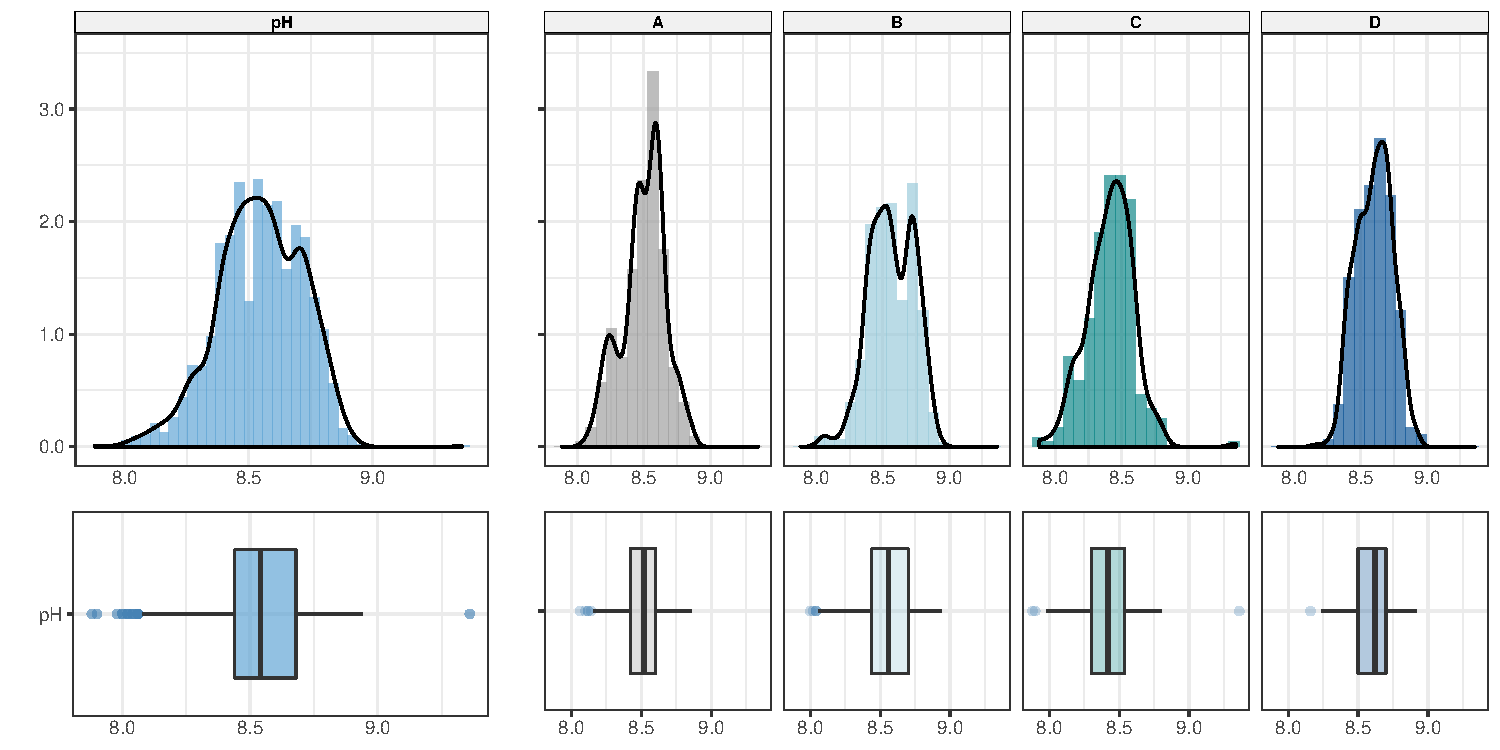
\includegraphics[width=1\textwidth]{Proj2-JM_files/figure-latex/unnamed-chunk-3-1} 

\caption{Distribution of Response Variable: pH}\label{fig:unnamed-chunk-3}
\end{wrapfigure}

Understanding the influence pH has on our predictors is key to building
an accurate predictive model. pH is a measure of acidity/alkalinity that
must conform in a critical range. The value of pH ranges from 0 to 14,
where 0 is acidic, 7 is neutral, and 14 is basic.

Figure 1.1 shows that our response distribution follows a somewhat
normal pattern and is centered around 8.5. The histogram for \texttt{pH}
is bimodal in the aggregate, but varies by brand. The boxplot view
allows us to better visualize the effect outliers have on the skewness
within our target variable.

Brand A has a negatively skewed, multimodal distribution, which could be
suggestive of several distinct underlying response patterns or a higher
degree of variation in \texttt{pH} response for this brand. The density
plot and histogram for Brand B show two bimodal peaks with a slight
positive skew. These peaks indicate that this brand has two distinct
response values that occur more frequently. The distribution for Brand C
and D are both more normal, with a slight negative skew. Brand D has the
highest median \texttt{pH} value and Brand C has the lowest. Brand C
also appears to have the largest spread of \texttt{pH} values.

\hypertarget{predictor-variables}{%
\section{Predictor Variables}\label{predictor-variables}}

We examined the density of our variables to visualize the distribution
of the predictors. Many of these variables contain outliers and present
with a skewed distribution. The outliers fall outside the red-line
boundaries, and highlight which predictors have heavier tails.

The density plots also contain an overlay of the only categorical
indicator, \texttt{BrandCode}. This view shows us that some variables,
including \texttt{AlchRel}, \texttt{CarbRel}, \texttt{CarbVolume},
\texttt{HydPressure4}, and \texttt{Tempature}, are strongly influenced
by brand type.

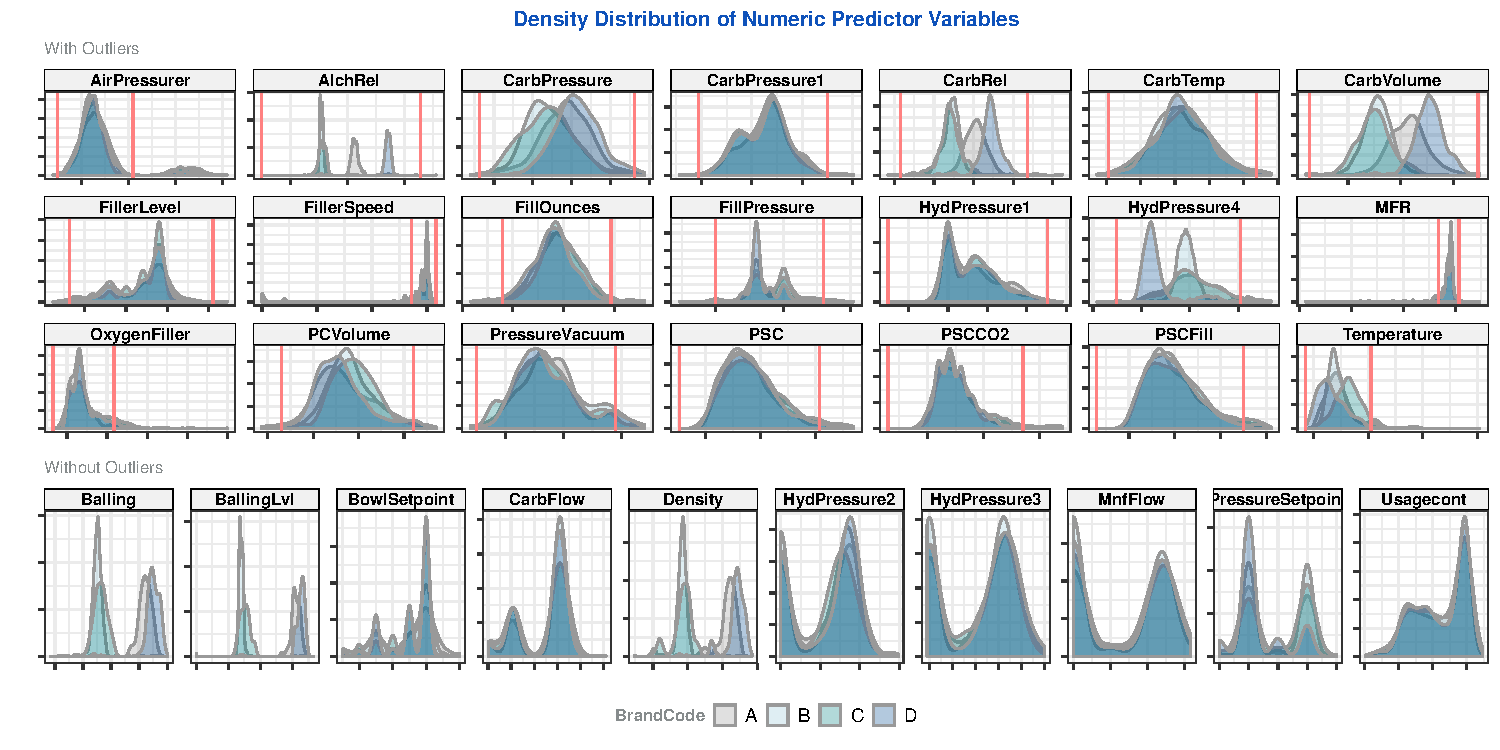
\includegraphics{Proj2-JM_files/figure-latex/unnamed-chunk-4-1.pdf}

We also looked at the relationship of our predictors against the
response variable below. There are a few predictors that have a weak,
linear association with our response variable. However, most of the
indicators show no strong patterns. Given these trends, we do not expect
linear modeling to provide optimal predictions for \texttt{pH}.

This view helps us further visualize the effect \texttt{BrandCode} has
on our predictor and \texttt{pH} values. For example, \texttt{AlchRel}
shows distinct \texttt{BrandCode} groupings. Other variables, such as
\texttt{PSCO2}, \texttt{BowlSetpoint}, \texttt{MinFlow}, and
\texttt{PressureSetup} show unique features likely related to system
processes.

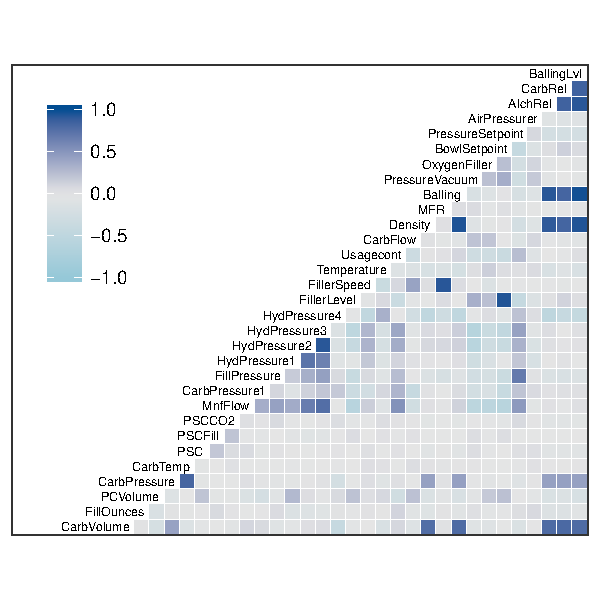
\includegraphics{Proj2-JM_files/figure-latex/unnamed-chunk-5-1.pdf}

Lastly, we examined collinearity measures between our numeric predictors
and found that several of these variables were heavily related, with
correlation values exceeding \(\pm{0.7}\).

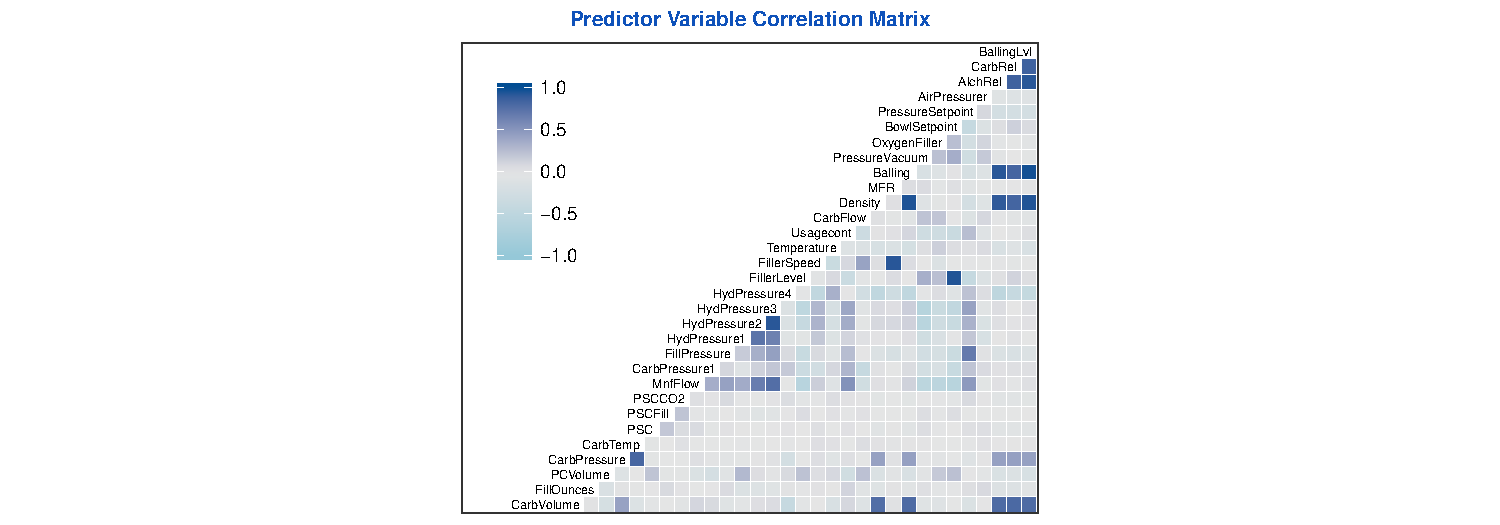
\includegraphics{Proj2-JM_files/figure-latex/unnamed-chunk-6-1.pdf}

\hypertarget{data-preparation}{%
\chapter{Data Preparation}\label{data-preparation}}

In our exploration, we detected missing data, extreme outliers, and
multicollinearity. We selected our modeling methods keeping these
factors in mind. Our approach included the application strategic
transformations to evaluate several types of non-linear and tree-based
modeling.

We divided the production dataset using an 80/20 split to create a train
and test set. All models incorporated k-folds cross-validation set at 10
folds to protect against overfitting the data. We set up unique model
tuning grids to find the optimal parameters for each regression type to
ensure the highest accuracy within our predictions.

\hypertarget{data-imputation}{%
\subsubsection{Data Imputation}\label{data-imputation}}

We choose to drop the complete cases of all \texttt{pH} observations
with null data in the target as they accounted for such a small
proportion (\textless{} 0.002\%) of the observations. We compared this
approach with other types of imputation and found that dropping
variables, in this instance, provided a slight boost within our accuracy
measures.

For our predictor variables, we applied a Multiple Imputation by Chained
Equations (MICE) algorthim to predict the missing data using sequential
regression. This method filled in all incomplete cases, including
\texttt{BrandCode}, our one unordered categorical variable.

\hypertarget{pre-processing}{%
\subsubsection{Pre-Processing}\label{pre-processing}}

Decision models trees are robust against these identifed issues. Thus,
requiring minimal data tranformation to properly evaluate our data. Our
non-linear models required more attention, so we incorporated variable
centering and scaling into the pre-processing to maximize their
performance.

We tested the effect of box-cox transformations on our non-linear and
tree-based models. The box-cox method changes the distribution shape of
our predictor variables, which normalizes the scale that they are
evaluated on. We found this transformation improve our modeling outcomes
in some instances.

\hypertarget{modeling}{%
\chapter{Modeling}\label{modeling}}

For our non-linear approach, we selected Support Vector Machines (SVM),
Multivariate Adaptive Regression Splines (MARS), and Elastic Net (eNet)
models. We compared these methods to tree-based regression using
gradient boosted models (GBM).

\hypertarget{svm}{%
\subsubsection{SVM}\label{svm}}

For SVM, we choose to work with a non-linear, radial kernel because many
of our data's features did not appear to be linearly separable. SVM
models work well in maintain a large amount of features and can make
distinctions between class differences.

Our RMSE Cross Validation plots show us that both models performed
similiary, but the second model performed slightly better. We choose
this model, which applied zero-varience, box-cox, centering, and spread
transformations, to be our preferred SVM model.

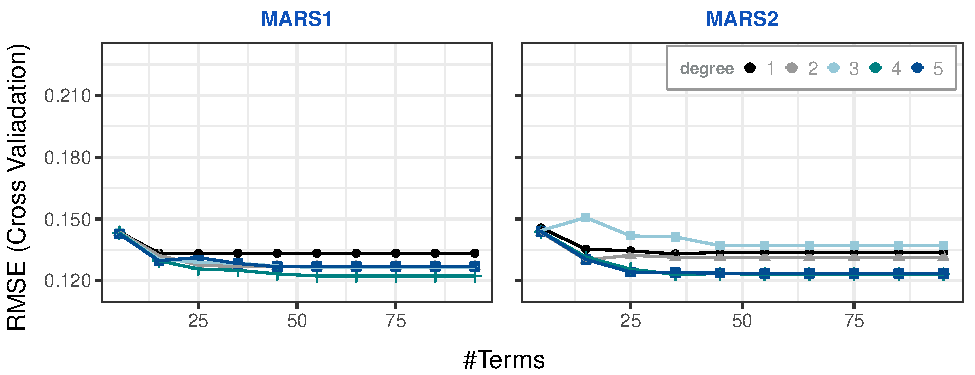
\includegraphics{Proj2-JM_files/figure-latex/unnamed-chunk-7-1.pdf}

\hypertarget{mars}{%
\subsubsection{MARS}\label{mars}}

MARS modeling was also selected to assess the non-linear features in our
data. This method uses a weighted sum to models nonlinearities and
interactions between variables. The model assesses cut-points between
features that create the smallest error and prunes insignificant points
to improve model accuracy.

Our RMSE Cross Validation plots show us that the best tune for both MARS
were very similiar. The second model, which contained box-cox
transformations, was selected as it performed the most consistently
across degrees and obtained a lower RMSE score.

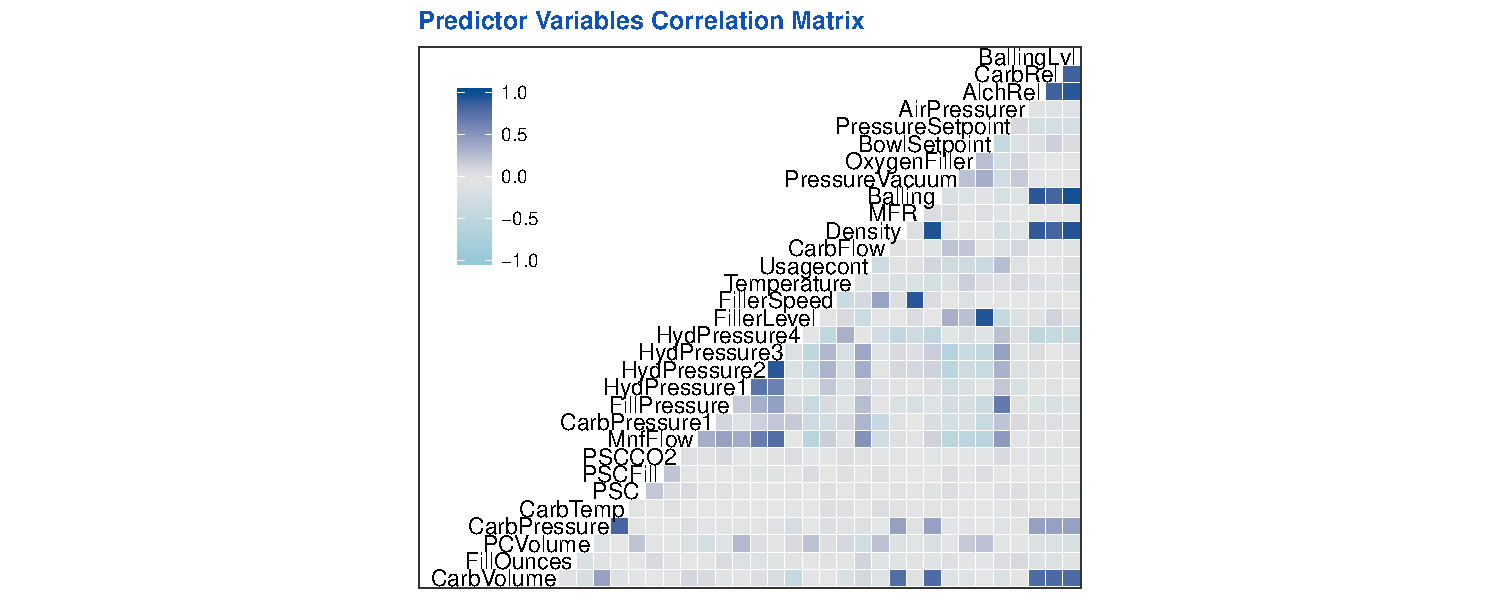
\includegraphics{Proj2-JM_files/figure-latex/unnamed-chunk-8-1.pdf}

\hypertarget{enet}{%
\subsubsection{eNET}\label{enet}}

The Elasticnet model was used as it can handle a large number of
predictor variables. It combines ridge and lasso regression techniques
to reduce the size of coefficients.

Our RMSE Cross Validation plots show us that the best tune for both eNET
were also similiar, with eNET1 performing slightly better. This model
center and scaled the data but did not apply a box-cox transformations.

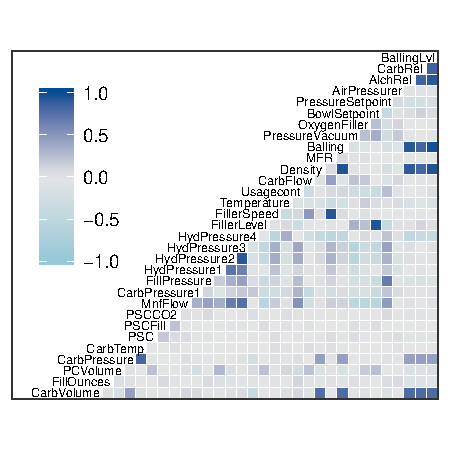
\includegraphics{Proj2-JM_files/figure-latex/unnamed-chunk-9-1.pdf}

\hypertarget{gbm}{%
\subsubsection{GBM}\label{gbm}}

Gradient boosting uses machine learning to train a prediction model
using decision trees. Our GBM used 1000 trees and was evaluated on a
grid using varying interaction depths, shrinkage, and terminal node
parameters.

We found that our second model with box-cox transformations help boosted
RMSE performance when the shrinkage size was 0.5. We choose the best
tune from the second model as our preferred model.

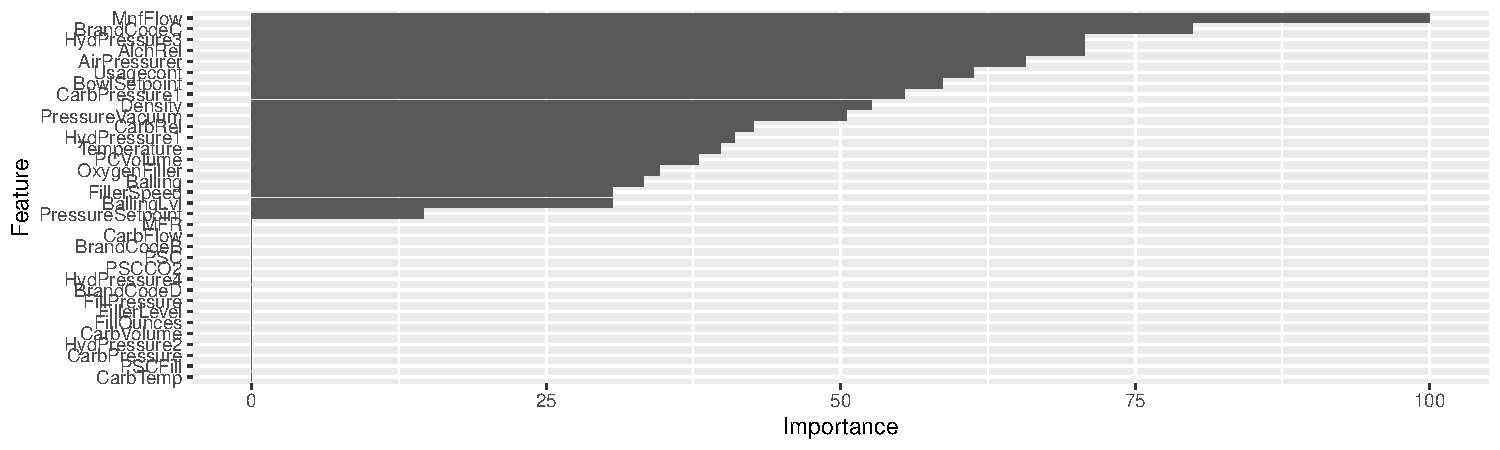
\includegraphics{Proj2-JM_files/figure-latex/unnamed-chunk-10-1.pdf}

\hypertarget{regression-analysis}{%
\chapter{Regression Analysis}\label{regression-analysis}}

This section will discuss the highlights and draw back of our tested
models. I am withholding content until we review and merge.

\hypertarget{accuracy}{%
\section{Accuracy}\label{accuracy}}

The SVM model achieved the highest accuracy measures for non-linear
modeling and the GBM model outperformed all of those other attempts.
Will add to a more indepth analysis of these metrics after the merge.

\begin{table}[H]

\caption{\label{tab:unnamed-chunk-11}Accuracy Measures}
\centering
\fontsize{8}{10}\selectfont
\begin{tabular}{lrrrrrr>{\bfseries\leavevmode\color{black}\columncolor[HTML]{B0DFe5}}r>{\bfseries\leavevmode\color{black}\columncolor[HTML]{B0DFe5}}r}
\toprule
  & SVM\_Train & SVM\_Test & MARS\_Train & MARS\_Test & eNET\_Train & eNET\_Test & GBM\_Train & GBM\_Test\\
\midrule
\rowcolor{gray!6}  RMSE & 0.12187 & 0.11057 & 0.12303 & 0.11669 & 0.13474 & 0.12594 & 0.10536 & 0.10347\\
Rsquared & 0.51456 & 0.55908 & 0.50555 & 0.52490 & 0.40186 & 0.42577 & 0.63554 & 0.61309\\
\rowcolor{gray!6}  MAE & 0.08861 & 0.08142 & 0.09286 & 0.08964 & 0.10515 & 0.09721 & 0.07820 & 0.07807\\
MAPE & 0.01110 & 0.00958 & 0.01142 & 0.01053 & 0.01297 & 0.01141 & 0.01021 & 0.00916\\
\bottomrule
\end{tabular}
\end{table}

\hypertarget{variable-importance}{%
\section{Variable Importance}\label{variable-importance}}

This section will discuss the trends in variable features in our
selected models. Below shows the top ten important variables by model.

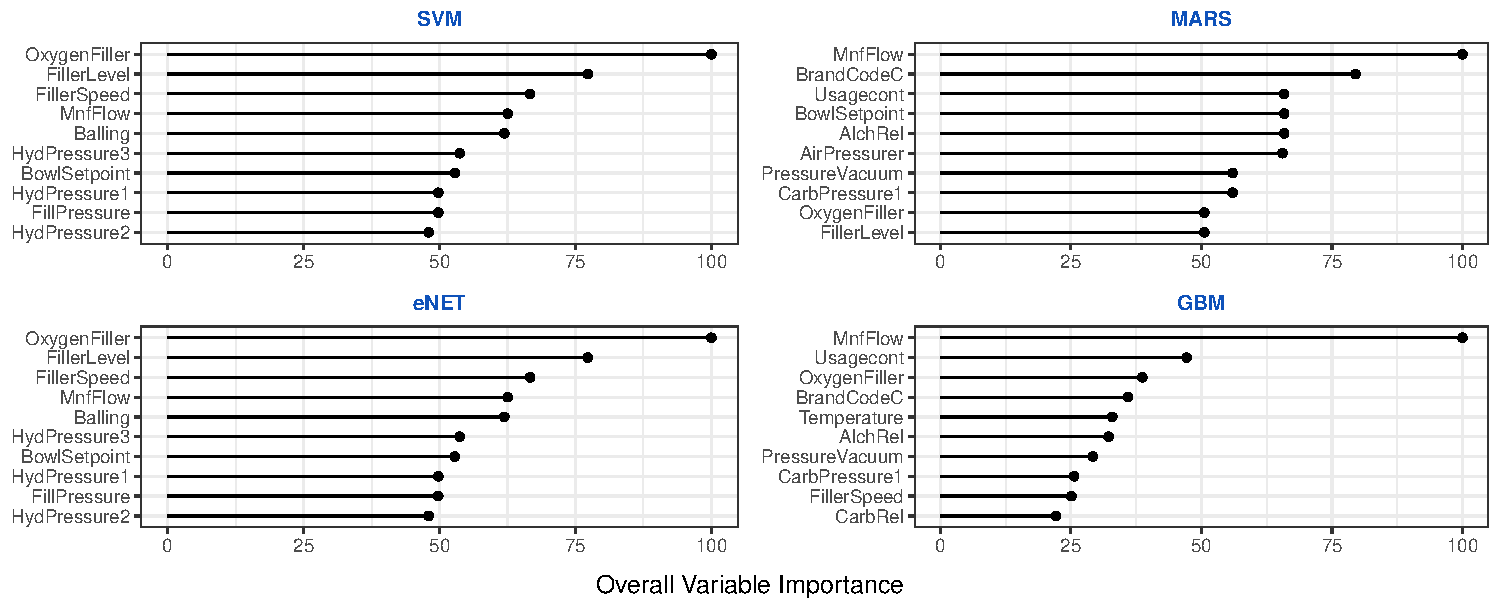
\includegraphics{Proj2-JM_files/figure-latex/unnamed-chunk-12-1.pdf}

\hypertarget{conclusion}{%
\chapter{Conclusion}\label{conclusion}}

I will save sprusing up this section once everyones models are live and
selected for final analysis.

\hypertarget{Appendix}{%
\chapter*{Appendix}\label{Appendix}}
\addcontentsline{toc}{chapter}{Appendix}

\hypertarget{summary-statistics}{%
\subsubsection{Summary Statistics}\label{summary-statistics}}

\begin{table}[H]
\centering\begingroup\fontsize{8}{10}\selectfont

\begin{tabular}{lrrrrrrrrrrrrr}
\toprule
  & vars & n & mean & sd & median & trimmed & mad & min & max & range & skew & kurtosis & se\\
\midrule
\rowcolor{gray!6}  BrandCode* & 1 & 2447 & 2.5 & 1.0 & 2.0 & 2.5 & 0.0 & 1.0 & 4.0 & 3.0 & 0.4 & -1.1 & 0.0\\
CarbVolume & 2 & 2557 & 5.4 & 0.1 & 5.3 & 5.4 & 0.1 & 5.0 & 5.7 & 0.7 & 0.4 & -0.5 & 0.0\\
\rowcolor{gray!6}  FillOunces & 3 & 2529 & 24.0 & 0.1 & 24.0 & 24.0 & 0.1 & 23.6 & 24.3 & 0.7 & 0.0 & 0.9 & 0.0\\
PCVolume & 4 & 2528 & 0.3 & 0.1 & 0.3 & 0.3 & 0.1 & 0.1 & 0.5 & 0.4 & 0.3 & 0.7 & 0.0\\
\rowcolor{gray!6}  CarbPressure & 5 & 2540 & 68.2 & 3.5 & 68.2 & 68.1 & 3.6 & 57.0 & 79.4 & 22.4 & 0.2 & 0.0 & 0.1\\
\addlinespace
CarbTemp & 6 & 2541 & 141.1 & 4.0 & 140.8 & 141.0 & 3.9 & 128.6 & 154.0 & 25.4 & 0.2 & 0.2 & 0.1\\
\rowcolor{gray!6}  PSC & 7 & 2534 & 0.1 & 0.0 & 0.1 & 0.1 & 0.0 & 0.0 & 0.3 & 0.3 & 0.9 & 0.7 & 0.0\\
PSCFill & 8 & 2544 & 0.2 & 0.1 & 0.2 & 0.2 & 0.1 & 0.0 & 0.6 & 0.6 & 0.9 & 0.8 & 0.0\\
\rowcolor{gray!6}  PSCCO2 & 9 & 2528 & 0.1 & 0.0 & 0.0 & 0.0 & 0.0 & 0.0 & 0.2 & 0.2 & 1.7 & 3.7 & 0.0\\
MnfFlow & 10 & 2567 & 24.6 & 119.5 & 70.2 & 21.1 & 161.6 & -100.2 & 229.4 & 329.6 & 0.0 & -1.9 & 2.4\\
\addlinespace
\rowcolor{gray!6}  CarbPressure1 & 11 & 2535 & 122.6 & 4.7 & 123.2 & 122.5 & 4.4 & 105.6 & 140.2 & 34.6 & 0.0 & 0.1 & 0.1\\
FillPressure & 12 & 2549 & 47.9 & 3.2 & 46.4 & 47.7 & 2.4 & 34.6 & 60.4 & 25.8 & 0.5 & 1.4 & 0.1\\
\rowcolor{gray!6}  HydPressure1 & 13 & 2556 & 12.5 & 12.4 & 11.4 & 10.9 & 16.9 & -0.8 & 58.0 & 58.8 & 0.8 & -0.1 & 0.2\\
HydPressure2 & 14 & 2552 & 21.0 & 16.4 & 28.6 & 21.1 & 13.3 & 0.0 & 59.4 & 59.4 & -0.3 & -1.6 & 0.3\\
\rowcolor{gray!6}  HydPressure3 & 15 & 2552 & 20.5 & 16.0 & 27.6 & 20.5 & 13.8 & -1.2 & 50.0 & 51.2 & -0.3 & -1.6 & 0.3\\
\addlinespace
HydPressure4 & 16 & 2539 & 96.3 & 13.1 & 96.0 & 95.5 & 11.9 & 62.0 & 142.0 & 80.0 & 0.6 & 0.6 & 0.3\\
\rowcolor{gray!6}  FillerLevel & 17 & 2551 & 109.3 & 15.7 & 118.4 & 111.0 & 9.2 & 55.8 & 161.2 & 105.4 & -0.8 & 0.0 & 0.3\\
FillerSpeed & 18 & 2513 & 3688.1 & 769.6 & 3982.0 & 3920.2 & 47.4 & 998.0 & 4030.0 & 3032.0 & -2.9 & 6.8 & 15.4\\
\rowcolor{gray!6}  Temperature & 19 & 2555 & 66.0 & 1.4 & 65.6 & 65.8 & 0.9 & 63.6 & 76.2 & 12.6 & 2.4 & 10.3 & 0.0\\
Usagecont & 20 & 2562 & 21.0 & 3.0 & 21.8 & 21.3 & 3.2 & 12.1 & 25.9 & 13.8 & -0.5 & -1.0 & 0.1\\
\addlinespace
\rowcolor{gray!6}  CarbFlow & 21 & 2565 & 2472.1 & 1070.4 & 3030.0 & 2604.2 & 323.2 & 26.0 & 5104.0 & 5078.0 & -1.0 & -0.6 & 21.1\\
Density & 22 & 2567 & 1.2 & 0.4 & 1.0 & 1.2 & 0.1 & 0.2 & 1.9 & 1.7 & 0.5 & -1.2 & 0.0\\
\rowcolor{gray!6}  MFR & 23 & 2359 & 704.0 & 73.9 & 724.0 & 718.2 & 15.4 & 31.4 & 868.6 & 837.2 & -5.1 & 30.5 & 1.5\\
Balling & 24 & 2567 & 2.2 & 0.9 & 1.6 & 2.1 & 0.4 & 0.2 & 4.0 & 3.9 & 0.6 & -1.4 & 0.0\\
\rowcolor{gray!6}  PressureVacuum & 25 & 2567 & -5.2 & 0.6 & -5.4 & -5.3 & 0.6 & -6.6 & -3.6 & 3.0 & 0.5 & 0.0 & 0.0\\
\addlinespace
PH & 26 & 2567 & 8.5 & 0.2 & 8.5 & 8.6 & 0.2 & 7.9 & 9.4 & 1.5 & -0.3 & 0.1 & 0.0\\
\rowcolor{gray!6}  OxygenFiller & 27 & 2556 & 0.0 & 0.0 & 0.0 & 0.0 & 0.0 & 0.0 & 0.4 & 0.4 & 2.4 & 8.8 & 0.0\\
BowlSetpoint & 28 & 2565 & 109.3 & 15.3 & 120.0 & 111.4 & 0.0 & 70.0 & 140.0 & 70.0 & -1.0 & -0.1 & 0.3\\
\rowcolor{gray!6}  PressureSetpoint & 29 & 2555 & 47.6 & 2.0 & 46.0 & 47.6 & 0.0 & 44.0 & 52.0 & 8.0 & 0.2 & -1.6 & 0.0\\
AirPressurer & 30 & 2567 & 142.8 & 1.2 & 142.6 & 142.6 & 0.6 & 140.8 & 148.2 & 7.4 & 2.3 & 4.7 & 0.0\\
\addlinespace
\rowcolor{gray!6}  AlchRel & 31 & 2560 & 6.9 & 0.5 & 6.6 & 6.8 & 0.1 & 5.3 & 8.6 & 3.3 & 0.9 & -0.9 & 0.0\\
CarbRel & 32 & 2559 & 5.4 & 0.1 & 5.4 & 5.4 & 0.1 & 5.0 & 6.1 & 1.1 & 0.5 & -0.3 & 0.0\\
\rowcolor{gray!6}  BallingLvl & 33 & 2566 & 2.1 & 0.9 & 1.5 & 2.0 & 0.2 & 0.0 & 3.7 & 3.7 & 0.6 & -1.5 & 0.0\\
\bottomrule
\end{tabular}
\endgroup{}
\end{table}

\hypertarget{code}{%
\subsubsection{Code}\label{code}}

\begin{Shaded}
\begin{Highlighting}[]
\CommentTok{# Final R Code Will Be Inserted Here}
\end{Highlighting}
\end{Shaded}


\end{document}
